
\chapter{Emulation}\label{ch:emulation}

\section{QEMU}

QEMU is an open-source emulator introduced by Fabrice Bellard in the year 2003 and available in most Linux distributions now. It is embedded in different virtualization tools as KVM and XEN, too. QEMU is well tested and contains all the necessary features for emulations of other architectures on alternative hardware. 
QEMU is a generic emulator for different system architectures. It can also be used for emulation of obsolete hardware \cite[~p.24]{Opsahl2013}. 
It has been extended for various architectures as x86, ARM, PowerPC, Sparc32, Sparc64, MIPS and s390x.
It is a processor emulator using binary translation \cite{Butt2011} which is executing and translating emulated instructions based on blocks. Each block comprises one entry and one exit point \cite[~p.5]{Wang2010}. 
The binary translation will be executed with the "Tiny Code Generator" (TCG) inside of QEMU. 
The TCG is a small compiler replacing GCC because of unlimited releases and code changes. The TCG is converting the blocks of target instructions into a standardized form. 
Subsequently, it has to be compiled for the host or target architecture. 
If a binary for a new target architecture is necessary, the frontend of TCG will be converted while QEMU is ported to a new architecture. 
The TCG integrates new code for the new host architecture in the background then. It is also dedicated to improving performance with avoiding repeated translations by buffering already translated code \cite{Cota2017}. 
The TCG takes care of the emulation of the guest processor running as a thread launched by QEMU. The memory of a quest is allocated during launch. Then that is mapped into the address space of the QEMU process  \cite[~p.29]{Opsahl2013}.\\
It is possible to run unmodified guest operating systems. The open-source projects can use any Linux distribution as their base operating system then because QEMU is integrated as a default package. 
QEMU does not emulate the entire hardware. That is only possible for the CPU. QEMU is used for emulations in this Bachelor Thesis.

\section{Full-System Emulation}

The full-system emulation emulates a whole system with hardware, the operating system (with the Linux kernel) and the userspace (with application processes). 
The system (hardware and operating system) will be translated unmodified. The condition of system emulation (compared to user mode emulation) is that you can run privileged instructions \cite[~p.2]{Butt2011}. This feature enables the translation of the unmodified target code on the operating system.
That all leads to a slowdown of the emulation in comparison to the user-mode emulation.
Additionally, this emulation can be used as an application development platform where specific hardware is not available. 
System emulation with emulated hardware is slower than a real machine because instructions should be executed directly in the guest hardware.  However, that has to be emulated in software. 
That implies multiple host instructions as a result because of the translation for a single guest instruction \cite[~p.1]{Tong2014}.
It is possible to reduce the supported and attached additional devices with additional options. The deactivation of a graphic card can be specified with \textbf{-nographic} as an example. Afterwards, less hardware has to be emulated, which has given a better performance.  \\
System emulation benefits from the virtualization support as KVM. In this case, CPU operations are not required to emulate.

\section{User-Mode Emulation}

The user-mode emulation does not emulate the whole system. It is faster than the full-system emulation because it does not engage so much hardware resources. Application processes can be run in QEMU with a minimal system for a specific application. 
This emulation type is working on a system call level. Therefore, the application has to be runnable as a single process executable itself. The emulator is using the Linux kernel to emulate system signal calls then. That can be managed by mapping system calls of the target system to an equivalent system call on the host with threading (with a separate virtual CPU) \cite{QEMU}. This process does not require the emulation of the full  memory  management  unit \cite[~p.2]{Butt2011}.
The user-mode emulation can run directly non-privileged instructions or is using system calls to ask for a selected service from the operating system. \\
The disadvantage of user-mode emulation is the only possibility to run single processes. Most services contain different applications with the result of multiple processes. Consequently, these applications need a full system emulation.


\section{Emulation of Alternative Architectures}

It is achievable to emulate alternative architectures on another hardware architecture. The package qemu-user-static has to be installed then, and the chosen architecture has to be registered in binfmt\_misc. binfmt\_misc is a kernel module. 
You can register other architectures within that, so that multiple other architectures can be run on one host. 
Not only QEMU can be used for system emulation. But also, container technologies as Docker include an integrated QEMU compatibility as an additional emulation feature for building images for other architectures. 
This technology has got the name \ref{BuildX}"BuildX". Accordingly, a hybrid virtualization approach is practicable with different virtualization and emulation technologies as with QEMU and Docker together. In this case, an external Linux kernel will be integrated into QEMU, and the application can be mounted via a loaded Docker image in a hard disk image. 
The Linux kernel is required for QEMU and should be built or downloaded (see \ref{LinuxKernel}"Fetching Linux Kernel Image").\\
The initrd should match the Linux kernel and is optional. It is used to start an init process together with the required test scripts. \\

\begin{figure}[H]
\centering
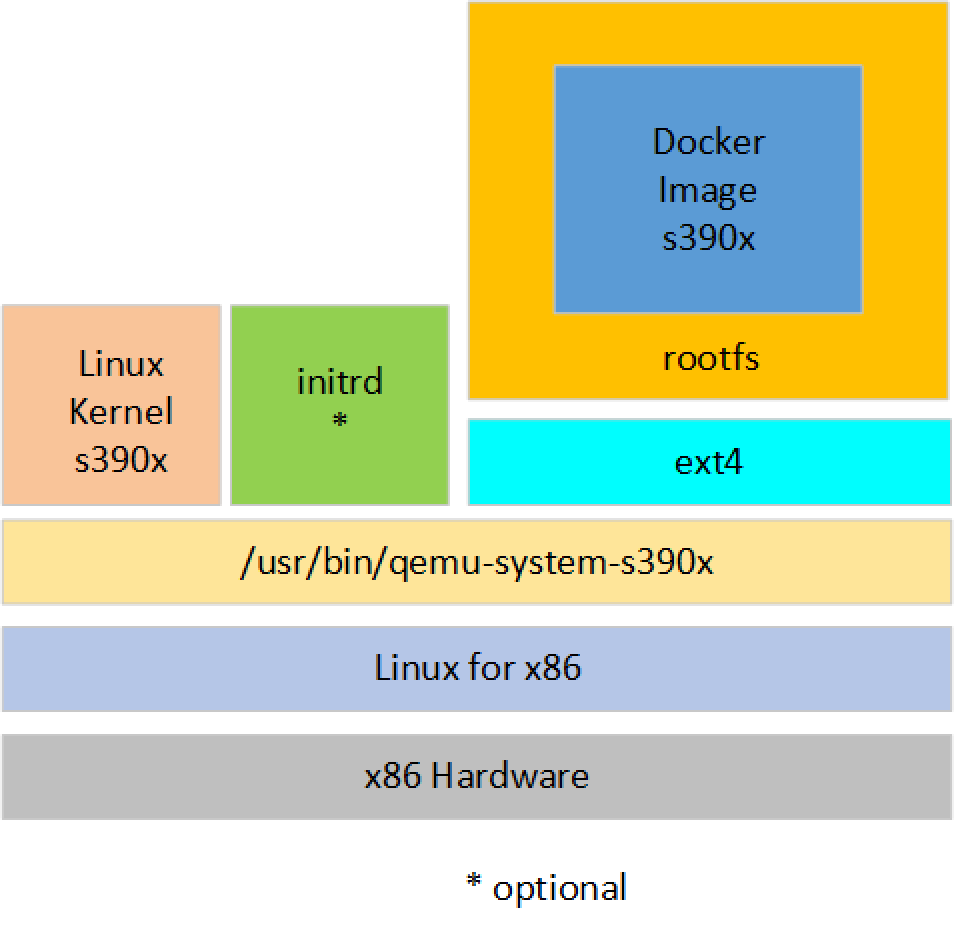
\includegraphics[height=9cm, width=9cm]{Qemu_setup}
 \caption{Emulation with QEMU}
    \label{QEMU_Emulation}
\end{figure}


\newpage
\subsection{Binfmt\_misc}

Binfmt\_misc is a kernel module which allows invoking almost every program by simply typing its name in the shell. That permits to execute user space applications such as emulators and virtual machines for other hardware architectures. It recognizes the binary-type by matching some bytes at the beginning of the file with a magic number. These executable formats have to be registered in the file \path{/proc/sys/fs/binfmt_misc/register}.\\
The structure of the configuration for the registration is the following: \\ \textbf{:name:type:offset:magic:mask:interpreter:flags} 

The \textbf{name} is the name of the architecture for the binary format. The \textbf{type} can be \textbf{E}, or \textbf{M}. E is for executable file formats as .exe for example. M is used for a format identified by a \textbf{magic} number at an absolute \textbf{offset} in the file, and the \textbf{mask} is a bitmask indicating which bits in the number are significant\cite{Slackware2020} (which is utilized in our case). 
The offset can be kept empty. The magic is a byte sequence of hexadecimal numbers. The \textbf{interpreter} is the program that should be invoked with the binary\cite{Guenther2020}. 
The path has to be specified for it. The field \textbf{flag} is optional. It checks different aspects of the invocation of the interpreter. The \textbf{F} flag is necessary in our case for "fix binary". 
That supposes that a new binary has to be spawned if the misc file format has been invoked.\\
In this way, it is possible to register another system architecture (s390x on x86) on the host system, and it is realizable to emulate the other architecture afterwards. \\
The necessary command for s390x registration can be found under \ref{Qemu-S390-Registration}.
The package \textbf{binfmt-support} has to be installed first for using this kernel feature. 

\subsection{Qemu-user-static}

The package \textbf{qemu-user-static}\footnote{\url{https://github.com/multiarch/qemu-user-static}} enables the execution of multi-architecture container emulation based on \textbf{binfmt\_misc} with \textbf{QEMU}. This package contained in various Linux distributions includes a set of binfmt configurations for various architectures together with an amount of statically compiled QEMU emulators that alternative architectures can run on another architecture \cite{Yang2019}. When building for one new architecture, static binaries are relevant because of the possibility of an "exec init error" without them. \\
The installation contains emulators for all available architectures supported by the QEMU project incl. s390x aligned with the specific host architecture. In this manner, you can build and run a binary for different architectures on the same host (see \ref{Optimized-Qemu-Command} Optimized Qemu Command). That is the base for \ref{BuildX}BuildX by Docker, too.

\subsection{BuildX}\label{BuildX}

As mentioned above, Docker is using QEMU for emulations with BuildX\footnote{\url{https://github.com/docker/buildx}}. That is an integrated "experimental Feature" since version Docker 19.03. That implies that it is not enabled as default because it is very new and for experiments. It has to be activated with \lstinline!DOCKER_CLI_EXPERIMENTAL=enabled! (see \ref{Qemu-S390-Registration} Registration of Qemu-S390x). The disadvantage of the provided BuildX inside of Docker is that you do not receive the up-to-date version of BuildX. There is a version with a more detailed output and better working with an additional \textbf{buildx} behind \textbf{docker build}. This version can be cloned from \url{https://github.com/docker/buildx} and installed with \textbf{make install}. \\
In general, BuildX is a Docker CLI plugin for expanding the "docker build" command. That includes the possibility of multi-architecture builds and exceptional output configuration. That involves not only the upload possibility to your local docker registry (see the output of \textbf{docker images}). That includes the output of "docker build" (which creates a docker image based on the requirements and installations in the used Dockerfile) into a local directory, a tar archive or a public registry on Docker Hub. Docker Hub is the most used and maintained registry for Docker images. \\
The \textbf{Dockerfile} is using the requirements by the base docker image in the FROM command on top of the Dockerfile together with installations and configurations executed by all RUN commands or attached scripts with the command ADD. The \textbf{-t} flag is adding a special name as a tag under \textbf{docker images}.
The special architecture for multi-architecture\ref{MultiArchitectureImages} builds can be specified with the additional option \textbf{--platform}.
The option \textbf{build create} provides the option to create different build instances for multiple build combinations of architectures.

\subsection{Multi-Architecture Images}\label{MultiArchitectureImages}

Default Linux distribution providers have to package their software for different system architectures because of different required drivers included in the Linux kernel and dependecies to these.
That is the reason that Docker images have to be built equally for different architectures. That can be performed with different base images for the respective architectures or with multi-arch images. 
It is possible to use one Dockerfile for different architectures then. One example for such a multi-arch Docker image is adoptopenjdk/adoptopenjdk8 based on Ubuntu\footnote{\url{https://github.com/AdoptOpenJDK/openjdk-docker/blob/master/8/jdk/ubuntu/Dockerfile.hotspot.nightly.full}}. In this case hardware dependencies are selected with \lstinline!dpkg --print-architecture! and included as ARCH into the different cases for downloading the relevant tar archive of OpenJDK:
\begin{figure}[H]
\centering
\begin{boxedverbatim}
RUN set -eux; \
    ARCH="$(dpkg --print-architecture)"; \
    case "${ARCH}" in \
       aarch64|arm64) \
         ESUM='2c6540ff8ea3d89362fd02143b24303e2359be249a6be6cb7e6580472686d863'; \
         BINARY_URL='https://github.com/AdoptOpenJDK/openjdk8-binaries/releases/
         download/jdk8u-2020-08-05-08-20/OpenJDK8U-jdk_aarch64_linux_hotspot_2020-
         08-05-08-20.tar.gz'; \
         ;; \
       armhf|armv7l) \
         ESUM='3c57c121415ef721ba9c73dfa809cd2f689d7369ef3d92d055f7c7c81ed2d697'; \
         BINARY_URL='https://github.com/AdoptOpenJDK/openjdk8-binaries/releases/
         download/jdk8u-2020-07-31-04-43/OpenJDK8U-jdk_arm_linux_hotspot_2020-07-
         31-04-43.tar.gz'; \
         ;; \
       ppc64el|ppc64le) \
         ESUM='668972e8d6d0815c03b32dac3f5c663453b4b0842938d13cfb0c1232a26a8087'; \
         BINARY_URL='https://github.com/AdoptOpenJDK/openjdk8-binaries/releases/
         download/jdk8u-2020-08-05-08-20/OpenJDK8U-jdk_ppc64le_linux_hotspot_2020-
         08-05-08-20.tar.gz'; \
         ;; \
       s390x) \
         ESUM='045aa287c48fd84eef19f2828ed1d15d27059a9328f5ca2cc91f6d42489af956'; \
         BINARY_URL='https://github.com/AdoptOpenJDK/openjdk8-binaries/releases/
         download/jdk8u-2020-08-05-08-20/OpenJDK8U-jdk_s390x_linux_hotspot_2020-
         08-05-08-20.tar.gz'; \
         ;; \
       amd64|x86_64) \
         ESUM='c26124b14c6a42d89278d3ce108b43c1210a317aba0163d985c06a79a695a174'; \
         BINARY_URL='https://github.com/AdoptOpenJDK/openjdk8-binaries/releases/
         download/jdk8u-2020-08-05-08-20/OpenJDK8U-jdk_x64_linux_hotspot_2020-08-
         05-08-20.tar.gz'; \
         ;; \
       *) \
         echo "Unsupported arch: ${ARCH}"; \
         exit 1; \
         ;; \
    esac; 
\end{boxedverbatim}
 \caption{Multi-Arch Image AdoptOpenJDK 8}
    \label{AdoptOpenJDK-Multi-Arch}
\end{figure}

You can see all URLs for arm64, armv7l, ppc64le, s390x and x86 in this case. This RUN command in the Dockerfile is using the architecture given by the option \\
\lstinline!--build-arg ARCH=s390x! \\
as an example in the \lstinline!docker build! command or the \lstinline!--platform! option will be used with BuildX.
\lstinline!Docker build! is stacked against BuildX, because only one image can be built with one command.
Buildx provides the possibility to consign different architectures (comma separated) to the platform option. Thereby, one command can build multiple images for different architectures.

\section{Filesystems}\label{FileSystems}

Docker is using the Union Filesystem which is not compatible with QEMU. \\
QEMU can integrate only hard disk formats for default Linux filesystems as ext2, ext3, ext4, XFS and Btrfs. 
The driver virtio\_blk is used to mount external filesystems and emulates read/write in the physical block device\cite{Barboza2018}. Following it, is possible to integrate and start nonnative systems in QEMU. 
Docker is advantageous to setup and start systems fast. 
It would be nice to integrate the docker filesystem into QEMU. After building a docker image, it is realizable to export the filesystem into a directory with the name \textbf{rootfs} with the command \\ 
\lstinline!docker export $(docker create initrd-s390x) | tar -C "rootfs" -xvf -!. \\

Linux has got the feature that it is adventitious to reformat directories for filesystems and to copy/ mount content into this one. Reformatting the default docker filesystem UnionFS to another one as ext4 for example can be done then. \\
QEMU is accepting the new filesystem as a block device for the guest system then. The default path to the mounted filesystem as a hard disk is \path{/dev/vda} for the first partition \cite[~p.22]{White2020}.

\subsection{UnionFS}\label{UnionFS}

Docker does not use any default Linux filesystem. 
Docker images are based on the Union Filesystem (UnionFS) \cite[~p.21]{Ashraf2015}. 
This filesystem is using different filesystem layers with grouping directories and files in branches. 
The first layer is the typical Linux boot filesystem with the name bootfs. 
That performs the same as in a Linux virtualization stack with using memory at first and unmounting to receiving RAM free by the initrd disk image. 
So the bootfs can be used inside of another Linux filesystem to mount in an virtualization stack for a successful boot process with QEMU.
The next layer contains the base image with the operating system given by the "FROM" command.
Then every docker command inside of the Dockerfile is adding an additional layer with the installation of applications or building binary files.
That is the reason that every executed docker command is receiving an own id in the disk memory during the build process.
Every separate docker command is using his own disk space. So a docker image can grow really fast.
It is reasonable to compress so much as possible of different routines into one docker command. 
All sizes of different docker layers will exist continuously inside of the new filesystem.

\begin{figure}[H]
\centering
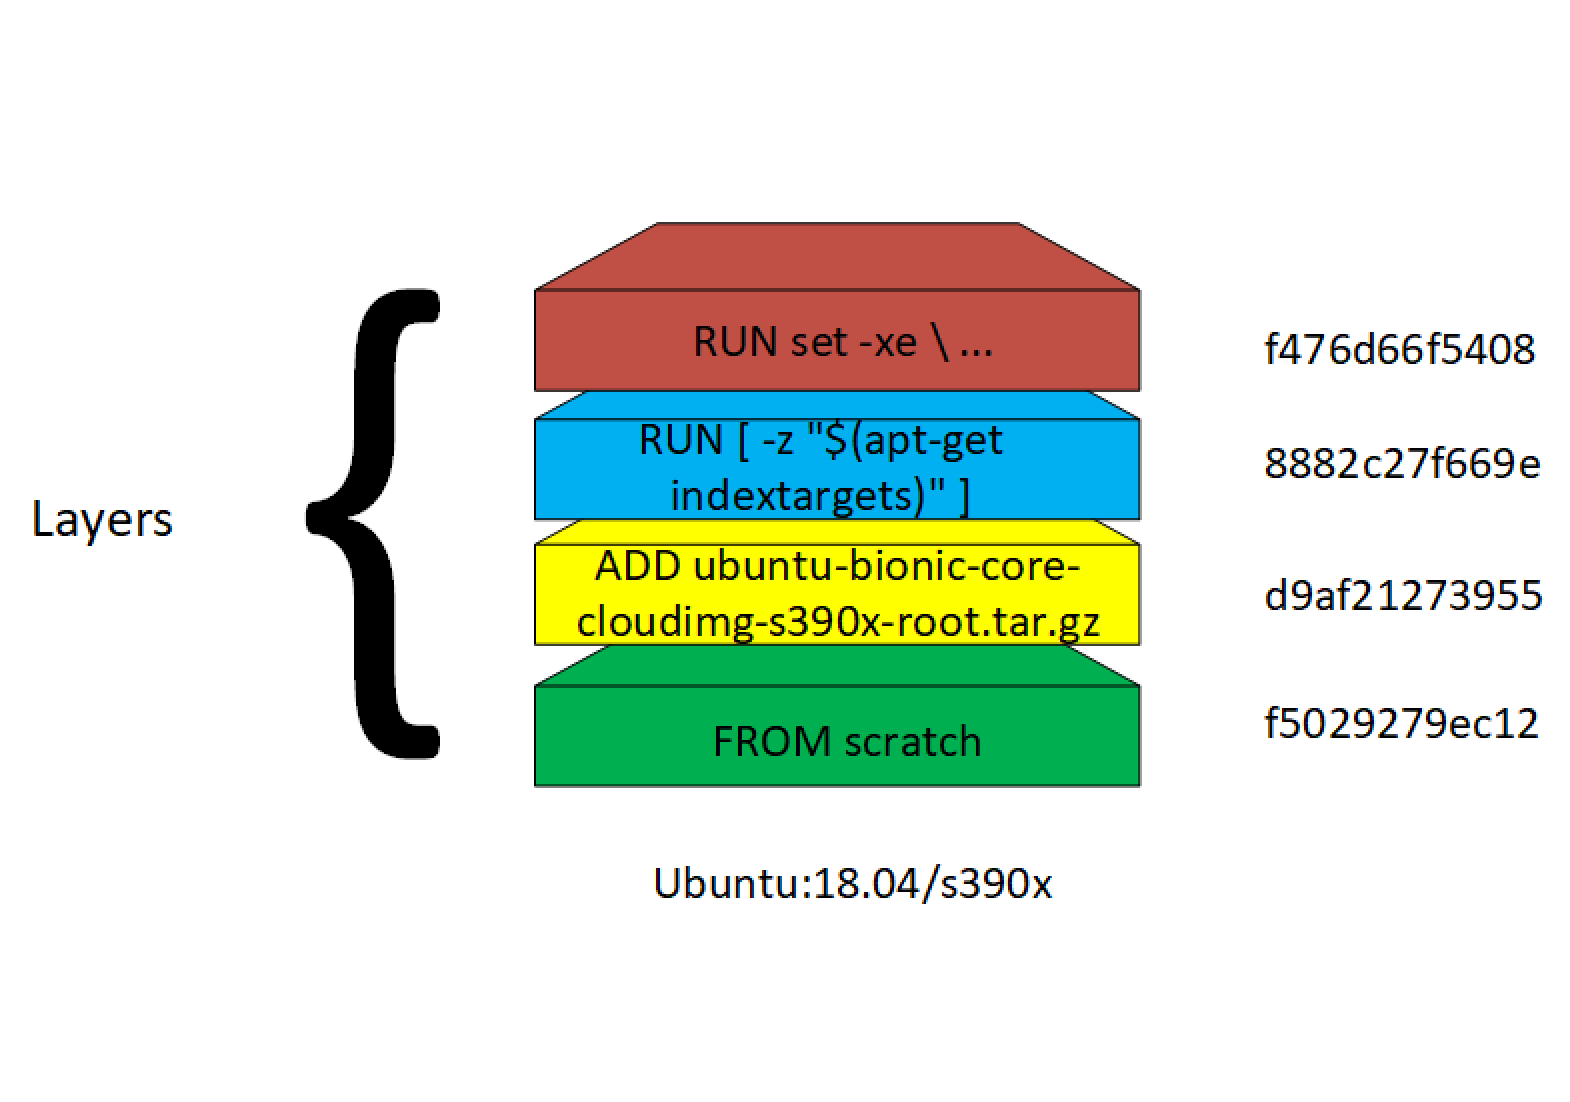
\includegraphics[width=\textwidth]{UnionFS}
 \caption{Union Filesystem}
    \label{UnionFS}
\end{figure}

\subsection{Ext4}

Ext4 is a journaling filesystem (equivalent to ext3). The journal is registering transactional all changes on the operating system with meta data.
So no data  are lost after a system failure. They can be restored based on the journal without a save procedure by the user.
Such journal filesystems in the ext filesystem family are working with blocks \cite[~p.20]{Seufert2015}.
The journal is splitted into the journal super block, descriptor blocks, commit blocks and revoke blocks.
The super block contains all meta data of the journal. Descriptor blocks include the special destination adress and a sequence number. 
Flex groups can combine multiple group blocks - inode bitmaps, inode tables and data blocks - to one logic block group. All data from inodes are only saved in the first flex group then. 
So the search for files is more powerful because meta data are allocated at one place.\\
All meta data from the journal can be relocated in inodes because changes of filesystem meta data are registered, too. \\
The difference to the journal in ext3 are the option writing asynchronous commit blocks and additional check sums for journal transactions \cite[~p.28]{Seufert2015}.

Ext4 provides a better performance than ext3. 
This filesystem can be formated with mkfs.ext4 which is available in every Linux distribution.
This tool is creating a group despriptor table for further group descriptors what allows an expanding of the filesystem. The filesystem can grow a maximum of the multiple 1024 of his existing size because of the saved space \cite[~p.21]{Seufert2015}. \\

Another feature of ext4 is the possibility of inline files and inline directories. So small files and directories can be saved directly in inodes instead of data blocks. From this follows less disk space consumption \cite[p.24]{Seufert2015}.

\begin{figure}[H]
\centering
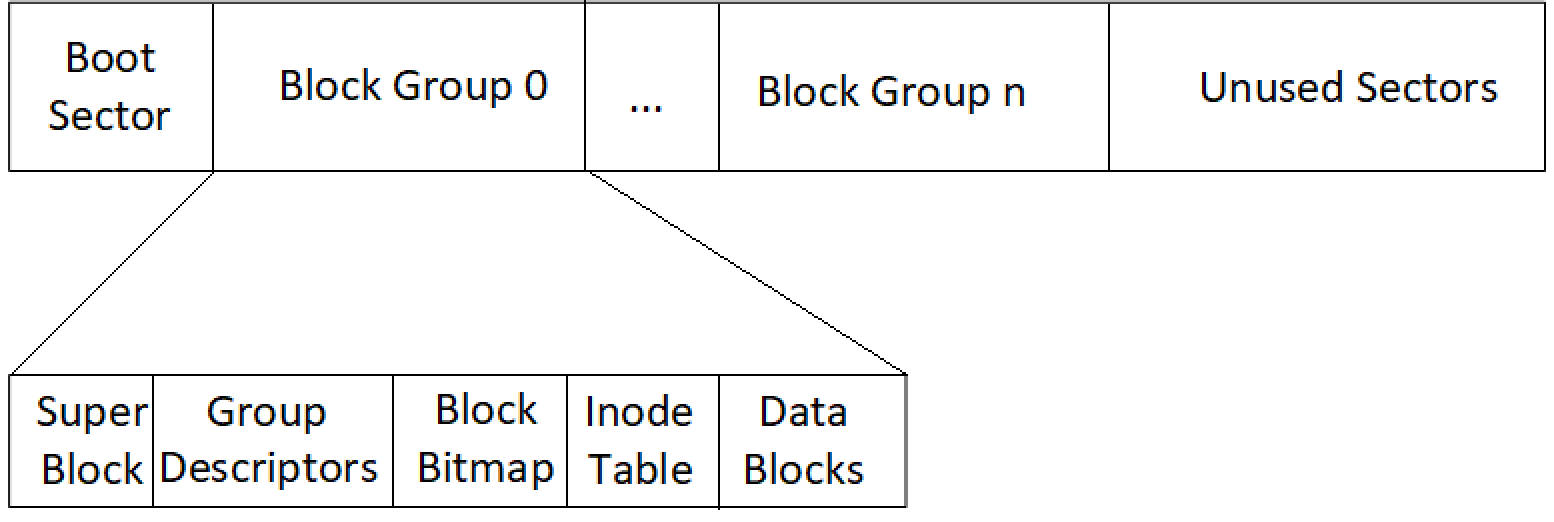
\includegraphics[width=\textwidth]{Ext4}
 \caption{Ext4}
    \label{Ext4}
\end{figure}

\subsection{Mounting an External Filesystem}

In \ref{FileSystems}"Filesystems" is described how to export a Docker filesystem into a directory. That has got the format of the \ref{UnionFS}"UnionFS" at this moment. QEMU contains the beneficial tool \textbf{qemu-img} for creating loadable images of filesystems. These require the minimal size of the docker image. The output of the size is given by \lstinline!docker images | grep ${id}!. Qemu-img understands only rounded numbers. Therefore, that has to be rounded up to a full number. That will be done automated with the tool \textbf{awk}. 
In the case of Cassandra, there will be used \\
\lstinline!docker images | grep 'Cassandra:s390x' | awk '{print int($7+0.5)"G"}'!. \\
\lstinline!print $7! would give the output of the size raw of \lstinline!docker images!, which is a float number. The \textbf{int} is rounding down to an integer number. Accordingly, the \textbf{0.5} has to be summed up for rounding up. The GB has been removed in this process. \lstinline!qemu-img! requires a G behind the number. That can be added with "G" inside of the awk command. \\

Finally, Cassandra is using the command \\
\lstinline!qemu-img create -f raw cassandra.img 2G! (see \ref{RunningDockerImage}"Running the Docker Image") \\
for the creation of a filesystem image with a Docker image size about 1.2G then. "2G" can be replaced by the command above in the CI/CD pipeline then (see \ref{CircleCI}"Circle CI configuration for Apache Cassandra"). \\
At first, cassandra.img is empty. The content of \textbf{rootfs} has to be transferred into this image file. But QEMU does not know UnionFS as a filesystem. That is the reason for formatting cassandra.img with \lstinline!mkfs.ext4 -F cassandra.img! to ext4. Writing into cassandra.img is only executible if the image is mounted into a directory under \path{/mnt/} with \\
\lstinline!mount -o loop cassandra.img /mnt/rootfs!. \\ 
In the next step the content of the filesystem directory can be copied into \path{/mnt/rootfs/} with \\ 
\lstinline!cp -r rootfs/* /mnt/rootfs/.!. \\ 
Then all data of the Docker image are saved into cassandra.img because it is mounted into \path{/mnt/rootfs/}. In conclusion, the image cassandra.img is usable for deployments with \textbf{qemu-system-s390x} (see \ref{RunCassandra} Run Cassandra). 